
\newcommand{\tsplot}{\textsc{Tsplot}}

\chapter{Time series visualization tool (\software{tsplot})} \label{chap:tsplot}
\renewcommand{\tabdir}{chapters/tsplot/tab}
\renewcommand{\figdir}{chapters/tsplot/fig}

%%%%%%%%%%%%%%%%%%%%%%%%%%%%%%%%%%%%%%%%%%%%%%%%%%%%%%%%%%%%%%%%%%%%%%%%%%%%%%%%
%%%%%%%%%%%%%%%%%%%%%%%%%%%%%%%%%%%%%%%%%%%%%%%%%%%%%%%%%%%%%%%%%%%%%%%%%%%%%%%%
%%%%%%%%%%%%%%%%%%%%%%%%%%%%%%%%%%%%%%%%%%%%%%%%%%%%%%%%%%%%%%%%%%%%%%%%%%%%%%%%
\section{Purpose} \label{sec:tsplot:purpose}
\software{tsplot} is a lightweight tool for the interactive visualization of time series data. It offers a convenient way to quickly inspect the output of an \software{echse}-based simulation model. It is particularly useful for showing simulated and observed data in a single plot for the purpose of comparison (see \figref{fig:tsplot:example}).
Note that \software{tsplot} is optimized for interactive plotting only. If you need to create plots for presentation in a paper, for example, you better use R commands or another software.

\begin{figure*}
  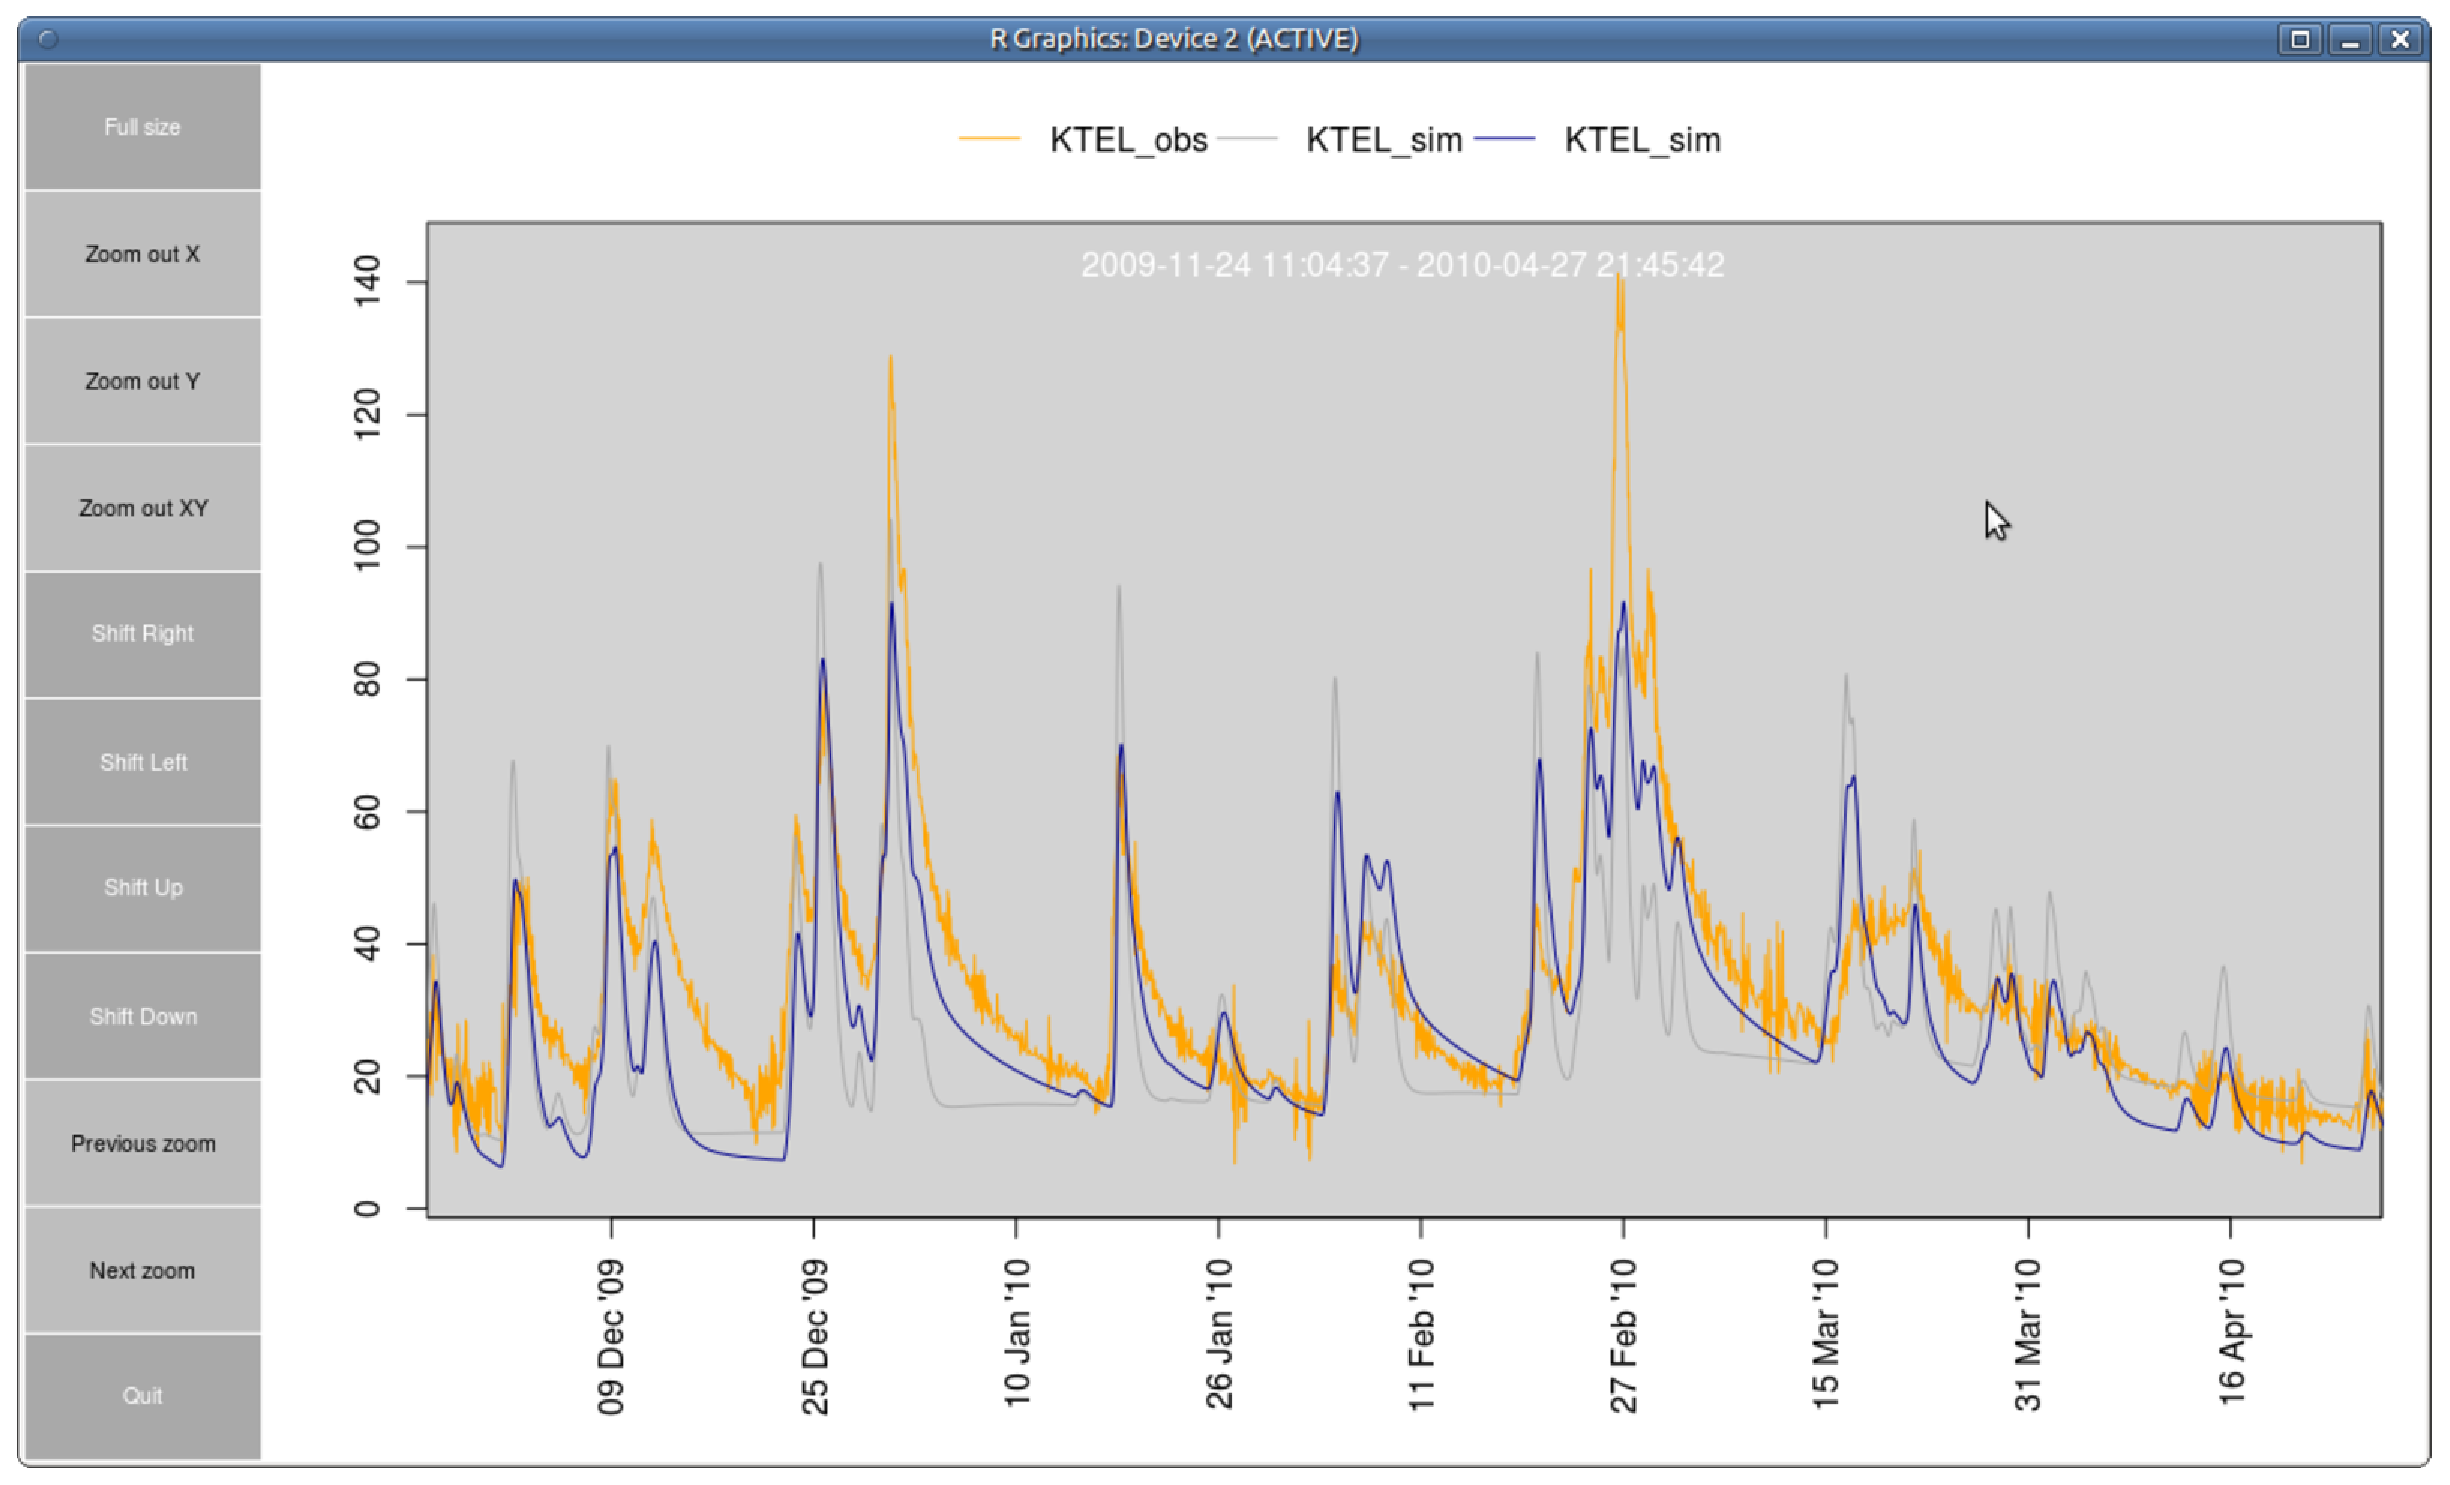
\includegraphics[width=0.9\textwidth]{\figdir/example.eps}
  \caption{Screen shot of a \software{tsplot} application. \label{fig:tsplot:example}}
\end{figure*}

%%%%%%%%%%%%%%%%%%%%%%%%%%%%%%%%%%%%%%%%%%%%%%%%%%%%%%%%%%%%%%%%%%%%%%%%%%%%%%%%
%%%%%%%%%%%%%%%%%%%%%%%%%%%%%%%%%%%%%%%%%%%%%%%%%%%%%%%%%%%%%%%%%%%%%%%%%%%%%%%%
%%%%%%%%%%%%%%%%%%%%%%%%%%%%%%%%%%%%%%%%%%%%%%%%%%%%%%%%%%%%%%%%%%%%%%%%%%%%%%%%
\section{Required software} \label{sec:tsplot:software}
\software{tsplot} is implemented as an R script. Thus, to use it, a current version of R must be installed. See \citet{Echse-Install-Doc} for information on how to install R. In order to invoke \software{tsplot} via a bash shell script under Windows, MSYS is required \citep[see][]{Echse-Install-Doc}.

%%%%%%%%%%%%%%%%%%%%%%%%%%%%%%%%%%%%%%%%%%%%%%%%%%%%%%%%%%%%%%%%%%%%%%%%%%%%%%%%
%%%%%%%%%%%%%%%%%%%%%%%%%%%%%%%%%%%%%%%%%%%%%%%%%%%%%%%%%%%%%%%%%%%%%%%%%%%%%%%%
%%%%%%%%%%%%%%%%%%%%%%%%%%%%%%%%%%%%%%%%%%%%%%%%%%%%%%%%%%%%%%%%%%%%%%%%%%%%%%%%
\section{Instructions files} \label{sec:tsplot:instructions}

The source(s) of the data to be plotted with \software{tsplot} and the corresponding styles are defined in instructions files. For every individual plot, one needs to create such a file. At a first glance, this may seem inconvenient. However, putting the instructions into a file allows for re-drawing a particular plot with only a single mouse click. In modeling studies -- and in particular during model calibration, when the data change frequently -- this is of great advantage.

Instruction files are plain text files containing data in a tabular format. The columns must be separated by white spaces (one or more spaces of tab characters). Each line of the file (row in the table) defines a time series to be plotted.

The instructions file must contain a table header with a complete set of column names (in any order). The meaning of the columns is as follows:
\begin{columndef}
  \item [file] (\textit{string}) Name of a text file containing time series data in the format described in \secref{sec:tsplot:datafiles}. Absolute or relative paths can be used. On Windows systems, it is important that the forward slash (\verb!/!) is used to separate the names of directories, instead of the usual backslash (\verb!\!).
  \item [colname] (\textit{string}) Name of a column existing in the data file specified in \texttt{file}. The values in this column are taken as the y-values. If the data file has no header, \ie{} no column names, one has to supply the index of the column rather than a name. The smallest useful index is 2 (see \secref{sec:tsplot:datafiles}).
  \item [color] (\textit{string}) Name of an existing color in R (examples: \emph{red} or \emph{lightblue}). Call the function \texttt{colors()} from an R prompt to display a (lengthy) list of all pre-defined color names.
  \item [type] (\textit{string}) This defines the style used for plotting. Using 'p' (for points) and 'l' (for lines) is appropriate for instantaneous data. For regular time series, where the values represent averages (or sums) over a intervals of time, you should 'S' or 's', depending on whether the given times specify the begin ('s') or the end ('S') of an interval. The output time series produced by \software{echse} models use the latter convention, thus you should use 'S'. Note that using 'p' may slow down the creation of plots significantly if the time series contain many values. In such cases, use one of the other options as an alternative.
  \item [name] (\textit{string}) A name for the series to appear in the legend.
  \item [header] (\textit{logical}) Must be a logical value (TRUE or FALSE in uppercase letters). If TRUE, \software{tsplot} expects the data file to contain a header with column names.
  \item [comment] (\textit{string}) A single character to be treated as a comment character in the data file. Quite often, the hash character (\verb!#!) is used for this purpose.
  \item [nodata] (\textit{string}) The value used in the data file to indicate missing values. Typical examples include 'NA' or '-9999'. The corresponding rows of the data file are ignored when creating the plot.
  \item [factor] (\textit{numeric}) A factor to be applied to the data before plotting. A value other that 1 may be useful to re-scale data when plotting multiple series whose values are of different magnitude.
  \item [xcut] (\textit{logical}) Must be a logical value (TRUE or FALSE in uppercase letters). If TRUE, the x-axis is truncated to the range of times contained in the data file. When plotting multiple series, a value of TRUE should not appear in more than 1 row of the instructions file.
\end{columndef}

An example of an instructions file is given in \figref{fig:tsplot:instructions-example}. If you need to put comment lines in the instructions file, use a semicolon as the first character of the line. The line will then be ignored by \software{tsplot} (see example in \figref{fig:tsplot:instructions-example}).

\begin{figure*}
  \lstinputlisting[style=txt]{\figdir/instructions-example.txt}
  \caption[Example of a \software{tsplot} instructions file.]{Example of a \software{tsplot} instructions file to display two time series of observed and simulated values. \label{fig:tsplot:instructions-example}}
\end{figure*}

%%%%%%%%%%%%%%%%%%%%%%%%%%%%%%%%%%%%%%%%%%%%%%%%%%%%%%%%%%%%%%%%%%%%%%%%%%%%%%%%
%%%%%%%%%%%%%%%%%%%%%%%%%%%%%%%%%%%%%%%%%%%%%%%%%%%%%%%%%%%%%%%%%%%%%%%%%%%%%%%%
%%%%%%%%%%%%%%%%%%%%%%%%%%%%%%%%%%%%%%%%%%%%%%%%%%%%%%%%%%%%%%%%%%%%%%%%%%%%%%%%
\section{Expected format of data files} \label{sec:tsplot:datafiles}
The actual time series data must be stored in plain text files. These file(s) must be formatted as follows:
\begin{itemize}
  \item A tabular format is expected with columns separated by the tab character (ASCII code 9).
  \item Time information must be in the \emph{first} column of the file.
  \item Times must be encoded as stings in ISO 8601 format (YYYY-MM-DD hh:mm:ss) with date and time separated by a single blank. Alternatively, one can provide only the date using the format YYYY-MM-DD. If only the date is given, a time of 00:00:00 is implicitly assumed.
  \item The times in column 1 may be given in regular \emph{or} irregular intervals. They should be in increasing order.
  \item The file can optionally have a header line specifying column names. Such names should be valid names in R, \ie{} the first character must be a letter. More letters, digits, and/or underscores may follow.
\end{itemize}

An example of a properly formatted time series file is shown in \figref{fig:tsplot:tseries-example}.

\begin{figure}
  \lstinputlisting[style=txt]{\figdir/tseries-example.txt}
  \caption{Example of a time series file for use with \software{tsplot}. \label{fig:tsplot:tseries-example}}
\end{figure}

%%%%%%%%%%%%%%%%%%%%%%%%%%%%%%%%%%%%%%%%%%%%%%%%%%%%%%%%%%%%%%%%%%%%%%%%%%%%%%%%
%%%%%%%%%%%%%%%%%%%%%%%%%%%%%%%%%%%%%%%%%%%%%%%%%%%%%%%%%%%%%%%%%%%%%%%%%%%%%%%%
%%%%%%%%%%%%%%%%%%%%%%%%%%%%%%%%%%%%%%%%%%%%%%%%%%%%%%%%%%%%%%%%%%%%%%%%%%%%%%%%
\section{Invoking \software{tsplot}} \label{sec:tsplot:invoke}

\subsection{On Linux} \label{sec:tsplot:invoke-linux}

On Linux, one needs to execute the shell script \texttt{tsplot.sh} and supply the name of the instructions file as a command line argument.

\subsubsection*{Using the command line}
Assuming that an instructions file \texttt{myplot.txt} exists in your home directory, a call from the command line might look as follows:

\begin{lstlisting}[style=shell]
  ./tsplot.sh /home/myname/myplot.txt
\end{lstlisting}

To use this, however, one first needs to navigate to the directory of \software{tsplot}, where the \texttt{tsplot.sh} resides. This is rather inconvenient. To be able to call \software{tsplot} from \emph{any} directory, you could do one of the following:

\begin{itemize}
  \item Move all files related to \software{tsplot} to a directory listed in the 'PATH' environment variable.
  \item Alternatively, add the path of the directory with the \software{tsplot} sources to the \verb!PATH! environment variable. See \citet{Echse-Install-Doc} for details.
  \item Alternatively, put a script in one of the directories already contained in the \verb!PATH! variable and let this script call \texttt{tsplot.sh}. In that case, you need to make sure that command line arguments are passed on.
\end{itemize}

\subsubsection*{Using the file browser's context menu}
In Ubuntu, Nautilus Actions provide the most convenient way to process an instructions file with \software{tsplot}. After defining a new action, you can simply process an instructions file from the Nautilus file browser's context menu. Thus, only two clicks with the right and left mouse buttons are necessary. See the documentation of Nautilus Actions for more info.

\subsection{On Windows} \label{sec:tsplot:invoke-windows}

On Windows, one needs to execute the batch file \texttt{tsplot.bat} and supply the name of the instructions file as a command line argument.

Assuming that an instructions file \verb!c:\temp\myplot.txt! exists, a call from the command line might look as follows:

\begin{lstlisting}[style=shell]
  tsplot.bat c:\temp\myplot.txt
\end{lstlisting}

To use this, however, one first needs to navigate to the directory of \software{tsplot}, where the \texttt{tsplot.bat} resides. To be able to call \software{tsplot} from \emph{any} directory, you could do one of the following:

\begin{itemize}
  \item Move all files related to \software{tsplot} to a directory listed in the \verb!path! environment variable.
  \item Alternatively, add the path of the directory with the \software{tsplot} sources to the \verb!path! environment variable. See \citet{Echse-Install-Doc} for details.
\end{itemize}

\subsubsection*{Using the file browser's context menu}
There are basically two ways:
\begin{itemize}
  \item Invent a new file extension for your instruction files (example: '.iii'). Create a new custom file type with that extension. Then configure the default 'open' action for the file type so that \texttt{tsplot.bat} is called with the file name as an argument. Thus, the 'open' action should read like \verb!some-path\tsplot.bat "%1"!.
  \item Alternatively, one can modify the 'open' action of any file type by editing the Windows registry. This is recommended for experienced users only and will not be described here.
\end{itemize}
